A common problem when defining modular theory hierarchies is that the most natural include-hierarchy for the most important theories is not necessarily the same as the most comprehensive hierarchy.
For example, Ex.~\ref{syn:incl} defines \cn{Group} with an include from \cn{Monoid}.
Instead, we could have used an intermediate theory and includes $\cn{Monoid}\harr \cn{CancellationMonoid}\harr\cn{Group}$.

It is very common to have increasingly strong theories $R,S,T$, where a design with two includes $R\harr S\harr T$ is not desirable:
\begin{compactitem}
 \item Often $R\harr T$ has been defined first and $S$ only later.
   This is very common because people usually formalize the most important theories (e.g., \cn{Monoid} and \cn{Group}) first.
   But inserting $S$ is not easy in retrospect --- changing the theory hierarchy (which is one of the most fundamental structures of a library) usually presents a very expensive refactoring problem.
   And even if we systematically use includes for every known intermediate theory like $S$ (as done in \cite{mathscheme}), we might later discover a new intermediate theory that should have been added.
 \item Often the most natural axioms to use in $T$ are the same independent of whether $T$ includes $R$ or $S$ (e.g., users might prefer the usual inverse-element axioms in \cn{Group} even if they have included \cn{CancellationMonoid}).
 In that case, the axioms of $S$ become provable in $T$ if we use $R\harr S\harr T$.
 This either causes $T$ to have redundant axioms or requires a more complex include mechanism that allows $T$ to include $S$ in a way that turns some of $S$-axioms into theorems.
\end{compactitem}

Therefore, it is common to use a commuting triangle consisting of two includes $R\harr T$ and $R\harr S$ and one morphism $m:S\to T$.
But this is awkward because the relation ``every $T$ is an $S$'' is now mediated by $m$ rather than being canonical.  
Implicit morphisms provide a simple solution to this problem: we keep the triangle but make the morphism $m$ implicit.
This captures exactly the canonical conversion from $S$ to $T$.

\begin{figure}[htb]
	\begin{center}
		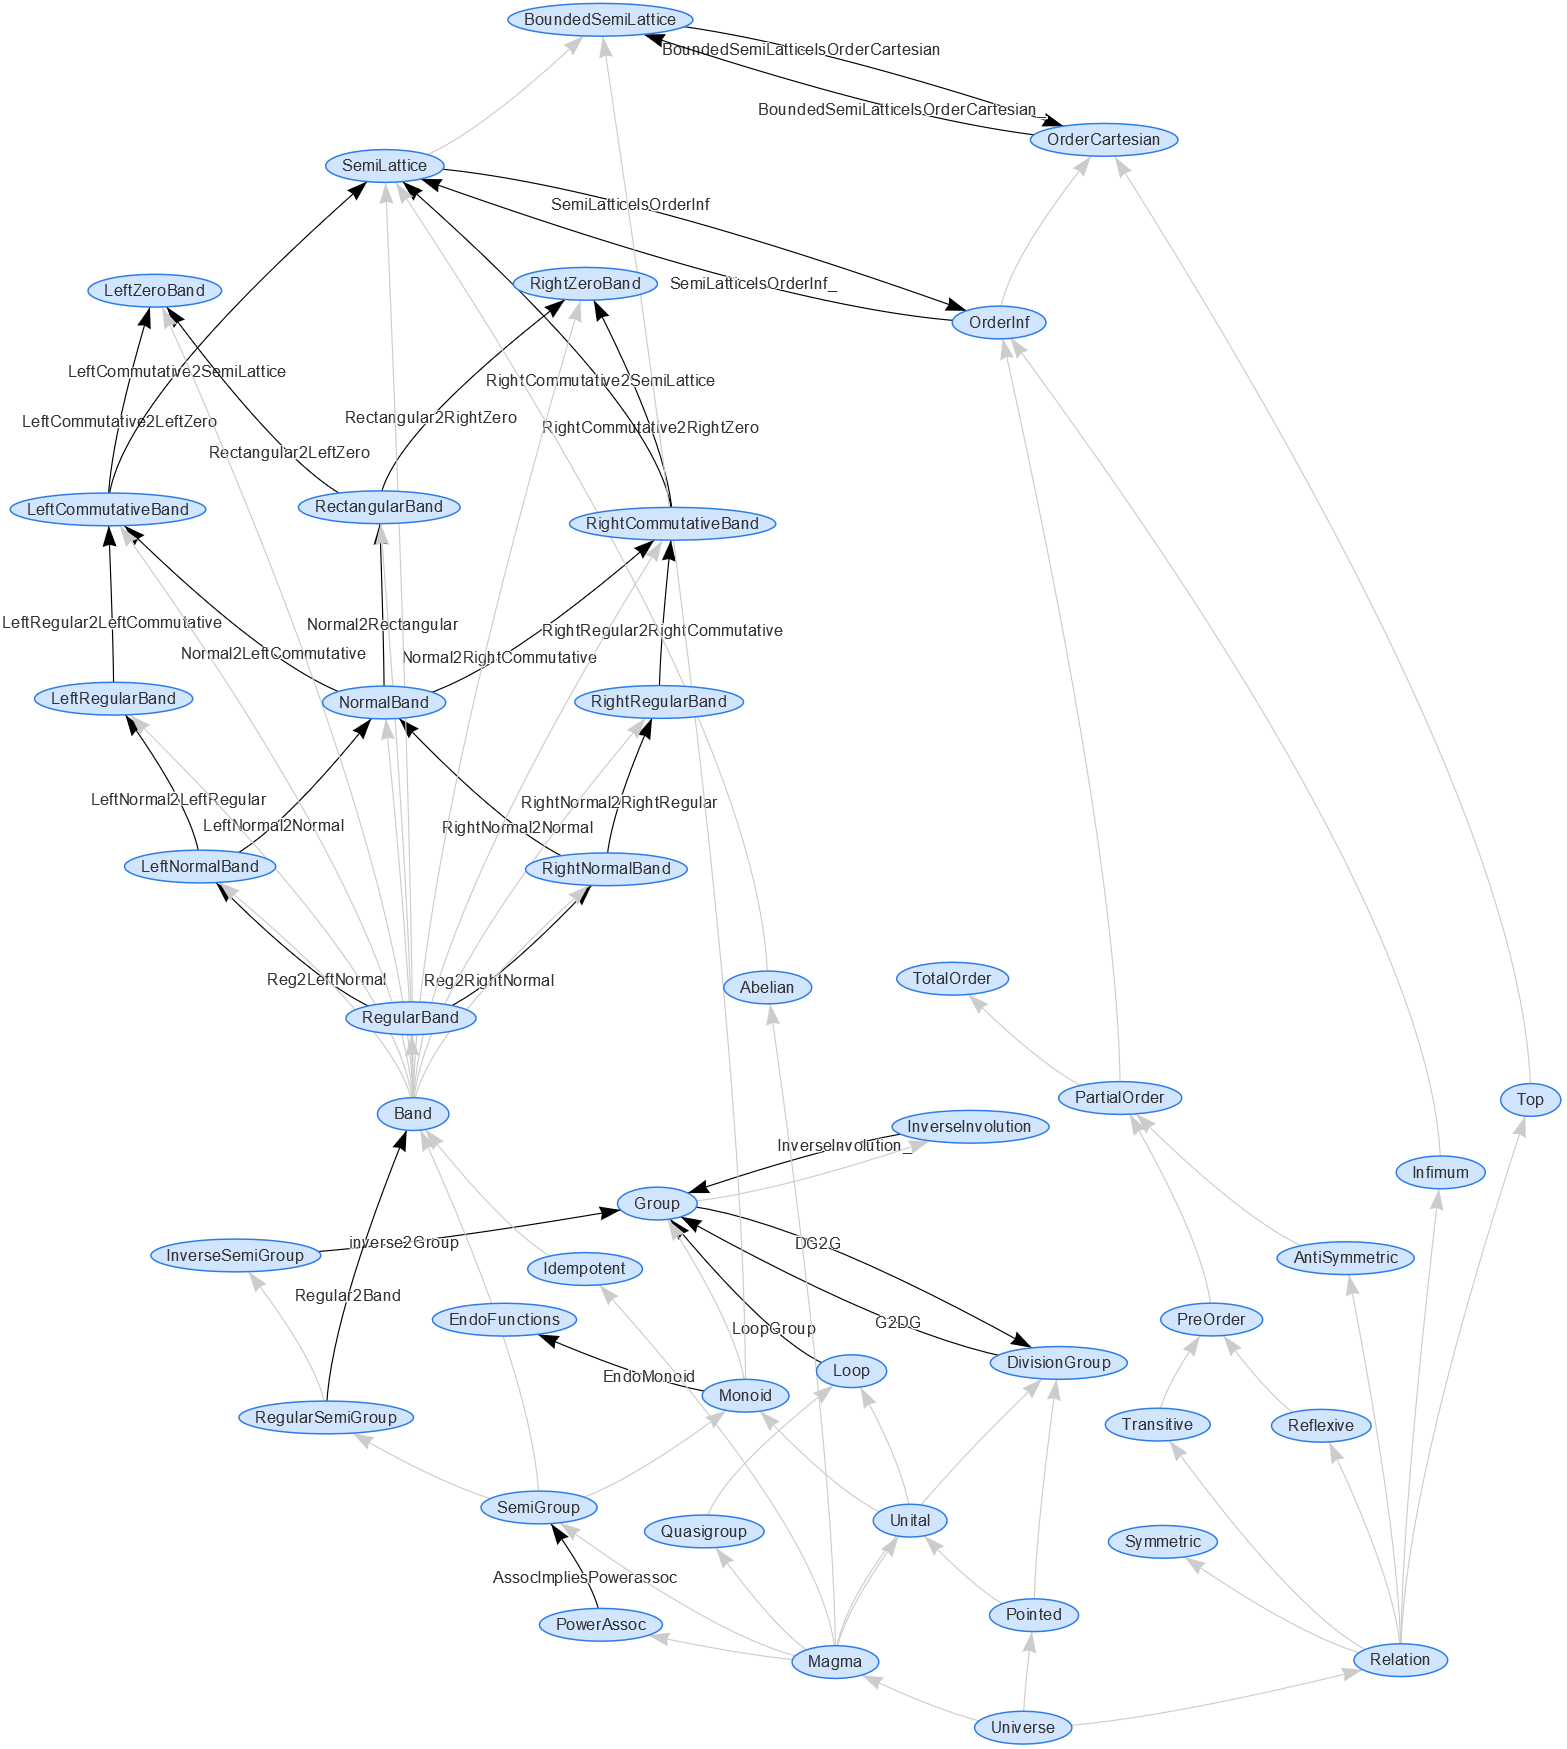
\includegraphics[width=.8\textwidth]{graph.png}
		\caption{Magma hierarchy with includes (gray) and implicit morphisms (black)}\label{fig:magmas}
	\end{center}
\end{figure}

Already the elementary algebraic hierarchy provides countless examples of such situations.
For a small fragment of the hierarchy of magmas, Figure~\ref{fig:magmas} shows one possible design using numerous implicit morphisms.
In particular, it uses some of the examples and features from this paper, e.g., an implicit isomorphism to identify the order-theoretic and the algebraic development of semilattices.

It also uses multiple implicit morphisms to introduce the various intermediate theories between $\cn{Band}\harr\cn{SemiLattice}$. 
All of these are of the form $t=\{\icl{\cn{Band}},\,a: F\}$, e.g., \cn{LeftRegularBand} uses $F=\forall x,z. z\circ x\circ z \doteq z\circ x$.
The implicit morphisms map the constants from \cn{Band} to themselves and the axiom $a$ to a proof.
It is straightforward to prove that this part of the diagram commutes: any two morphisms are identical except for the assignment to the axiom $a$, and these are equal due to proof irrelevance.%
\footnote{Our formalization of bands can be found at \url{https://gl.mathhub.info/MMT/examples/blob/devel/source/bands.mmt}.}
%\footnote{All varieties of bands can be axiomatized in this way.}


%\begin{center}
%\begin{tikzpicture}[xscale=2]
%  \node (s1) at (0,0) {$z\circ x\circ y\circ z\doteq  z\circ x\circ z\circ y\circ z$};
%  
%  \node (s2a) at (-1,-1) {$z\circ x\circ y\doteq  z\circ x\circ z\circ y$};
%  \node (s2b) at (1,-1) {$y\circ x\circ z\doteq  y\circ z\circ x\circ z$};
%  \draw[arrow] (s1) to (s2a) {};
%  \draw[arrow] (s1) to (s2b) {};
%  
%  \node (s3a) at (-2,-2) {$x\circ y\doteq  x\circ y\circ x$};
%  \node (s3b) at (0,-2) {$z\circ x\circ y\circ z\doteq  z\circ y\circ x\circ z$};
%  \node (s3c) at (2,-2) {$x\circ y\doteq  y\circ x\circ y$};
%  \draw[arrow] (s2a) to (s3a) {};
%  \draw[arrow] (s2a) to (s3b) {};
%  \draw[arrow] (s2b) to (s3b) {};
%  \draw[arrow] (s2b) to (s3c) {};
%  
%  \node (s4a) at (-1,-3) {$z\circ x\circ y\doteq  z\circ y\circ x$};
%  \node (s4b) at (1,-3) {$x\circ y\circ z\doteq  y\circ x\circ z$};
%  \draw[arrow] (s3a) to (s4a) {};
%  \draw[arrow] (s3b) to (s4a) {};
%  \draw[arrow] (s3b) to (s4b) {};
%  \draw[arrow] (s3c) to (s4b) {};
%
%  \node (s5) at (0,-4) {$x\circ y\doteq  y\circ x$};
%  \draw[arrow] (s4a) to (s5) {};
%  \draw[arrow] (s4b) to (s5) {};
% 
%  %\node[thy,inner sep=.3cm,fill=gray] (t1) at (0,0) {};
%  %\node at (t1.north west) {$S$};
%  %\node at (t1) {$D$};
%  %\node[thy,inner sep=.5cm,fill=lightgray] (s2) at (2,0) {};
%  %\node[thy,inner sep=.3cm,fill=gray] (t2) at (2,0) {};
%  %\node at (t2.north west) {$T$};
%  %\node at (t2) {$C$};
%  %\draw[view] (t1) to[out=10,in=170] node[above] {$\sigma$} (t2);
%\end{tikzpicture}
%\end{center}

%\begin{figure}
%\begin{tabular}{c|c}
%\begin{mmtcode}
%Band =
%  include ?SemiGroup
%  axiom_idemp : ⊦ ∀[x] x ∘ x ≐ x
%❚
%
%Regular =
%  include ?Band
%  axiom_regular : ⊦ ∀[x]∀[y]∀[z] 
%    z ∘ x ∘ z ∘ y ∘ z ≐ z ∘ x ∘ y ∘ z
%❚
%
%LeftNormal =
%  include ?Band
%  axiom_leftnormal : ⊦ ∀[x]∀[y]∀[z] 
%    z ∘ x ∘ z ∘ y ≐ z ∘ x ∘ y
%
%theory RightNormal =
%  include ?Band ❙
%  axiom_rightnormal : ⊦ ∀[x]∀[y]∀[z] 
%    y ∘ z ∘ x ∘ z ≐ y ∘ x ∘ z ❙ 
%❚
%
%theory Normal : ?Meta =
%  include ?Band ❙
%  axiom_normal :  ⊦ ∀[x]∀[y]∀[z] 
%    z ∘ x ∘ y ∘ z ≐ z ∘ y ∘ x ∘ z ❙
%❚
%\end{mmtcode} &
%\begin{mmtcode}
%implicit view Reg2LeftNormal : 
%    ?Regular -> ?LeftNormal =
%  include ?Band = ?Band ❙
%  axiom_regular = sketch "trivial" ❙
%❚
%
%implicit view Reg2RightNormal : 
%    ?Regular -> ?RightNormal =
%  include ?Band = ?Band ❙
%  axiom_regular = sketch "trivial" ❙
%❚
%
%implicit view LeftNormal2Normal : 
%    ?LeftNormal -> ?Normal =
%  include ?Band = ?Band ❙
%  axiom_leftnormal = sketch "trivial" ❙
%❚
%
%implicit view RightNormal2Normal : 
%    ?RightNormal -> ?Normal =
%  include ?Band = ?Band ❙
%  axiom_rightnormal = sketch "trivial" ❙
%❚
%\end{mmtcode}
%\end{tabular}
%
%\caption{Exemplary Theories for Some Varieties of Bands}\label{fig:bandsmmt}
%\end{figure}